\chapter{Introduction}\label{chap:01}
\begin{chapter-abstract}
Here I give an overview on my thesis.
This includes general topic and field of research (perceptual quality judgment that relies on memorization and then recall).
I state why this topic is relevant and what practical implications occur.
I give a brief overview on "service basics": to service, satisfaction, acceptance, money stuff.
At the end I will state the research questions and my approach towards answering this question.
I will give hints on the results a reader can expect.
\end{chapter-abstract}

%\section{Basic definitions}
%\item What is \emph{to service}? [Whitepaper] [http://www.merriam-webster.com/dictionary/service] 
%\item What is a service, application, system?
%\item Telecommunication services + Service Provider %https://www.law.cornell.edu/uscode/text/47/153#50

%\paragraph*{Service provider's goal}
%Make customer happy for as little money as possible for infrastructure: 
%\begin{itemize}
%\item cost-efficiency: trade-off
%\item risk reduction
%\item Service usage
%\item repeated usage / churn

%\item QoE as hygienic factor [Moeller, Wechsung]  
%\item Money: NPS, Churn, Acceptability, Willingness-to-paying
%\item Retainability (sMOS)
%\item Adaptive services: service that adjust performance to current conditions (best + economic feasible)
%\end{itemize}

\section{Motivation}
In difference to products, which can be manufactured and stored, is a service volatile.
A service is simultaneously produced or rather provided by the \emph{service provider} and consumed by the \emph{customer}.
A typical example is a \emph{telecommunication service} like speech telephony, or Internet access.
%US Communications Act 1934
Telecommunication services provide communication, \ie data transmission, between one or more parties.
Here a party can be a person but also a computer.
A service provider maintains the network infrastructure to provide those services and makes it available to potential users\footnote{Throughout this a person engaging a service is called \emph{user} of this service without distinction if he is the actual customer.}.
The actual service is produced, when a user uses a provided service, using the provider's network infrastructure for data transmission.

As a service is produced when it is used, the \emph{service performance} might be varying.
Here, service performance are absolutely measurable parameters of this service like transmission bandwidth and one-way transmission delay~\citep[cf][p. 12]{moller_assessment_2000}.
In case of a telecommunication service varying service performance can be the result of current network load conditions, network equipment failure, but also related to end-user devices (\eg the telephone) and other factors.
Usage of telecommunication services can be divided into two aspects.
First, a user can actively interact with a service like starting and engaging a telephone conversation.
Second, user can passively use a service, which provides like reachability of a telephone.

The active use by a user of a telecommunication service also results in a \emph{perceived quality} of this interaction (cf. \autoref{chap:02}).
It is assumed that perceived quality results from a comparison between the \emph{desired experience} and \emph{actual experience}. %Expected experience?
Here experience includes all perceptions resulting from this service instance \citep[cf.][p.13]{Book chapter 2}.
The perceived quality of an interaction with a service is affected by the experienced service performance, but also individual factors.

%QoE Methods; human perception 
Understanding the relationship between service (or system) performance with perceived quality has become important field of research.
Starting from speech transmission for telephony \citep[cf.]{IEEE Recommended Practice for Speech Quality Measurements} and the resulting degradations, perceived quality now mainly considers digital transmission of multimedia data \citep{moeller_quality_2015}}.
This includes the production, transmission (especially lossy coding) and reproduction of text, voice, speech, image and video information.
Specific characteristics of human perceptual system have been used to develop enhanced coding mechanisms like \ac{MP3} or \ac{H264}.
%Service choice!

\section{Research Questions}
This work extends prior work by investigating the impact of varying service/system performance on the perceived quality, when the same system(s) are used repeatedly.
This is, in fact, a common case for telecommunication service.
For example a customer of a mobile  provider will use the provided service(s) usually repeatedly, because his telephone number is bound to the service provider and, although it can be transfered to a different provider, this process takes time and effort.
Furthermore, a customer might be bound for a certain extend to a service provider contract duration.

The performance of a service might be varying from usage instance to usage instance.
From a user's perspective this might be sufficient, but if the performance some usage instances does meet the expectations / desired performance then a dissatisfaction might occur.
This force the user to abandon the service provider and chose a different one.

%TODO: Performance cannot be determined beforehand! Trust; Service usage lifecycle? Customer Expectations and providers promise

Before actually deciding to use a service, a potential user must have a need that can be fulfilled by using a service. %proposes to fulfill
If multiple service provider that provide a similar service, a potential user must chose which service to use for fulfillment of his need.
When satisfied with the outcome of using the service a user might interact with the service later on again, whereas a non-satisfying outcome will likely result in not using the same service again and rather use a different one.
In fact, using the same service again, saves time and resource, because the service discovery, evaluation and selection is not conducted.

Although contract duration might bind customers to a provider, low performance and thus a low perceived quality affects the future use behavior and increases the churn rate for the end of contract.
In addition, satisfaction and also dissatisfaction of a customers can spread to other customers and potential customers and thus have severe impact on the business performance of a service provider.

\section{Goals}
In this work I focus on the development of perceived quality over several distinct interactions with a telecommunication service and how a retrospective assessment of the perceived quality of this service is affected by varying service performance.
%TODO What is performance and what is perceived quality
The actual impact on customer satisfaction and thus business performance of performance variation is not in the scope of this thesis.

Two research questions are addressed in this thesis:
\begin{itemize}
\item How does perceptual quality evolve over multiple distinct interactions with the one system/service for one user?
\item How does perceptual quality evolve over multiple distinct interactions with a multiple services offered by the same service provider for one user?
\end{itemize}

Here distinct interaction refers to one usage instance by a user with a service to fulfill a certain need of the user or solve a certain task.
Such an instance is denoted as a \emph{usage episode}.
Each usage episode has a perceived quality, which can be assessed momentary while in the usage episode and also in retrospective after the usage episode is finished.
In this thesis I investigate how a multi-episodic perceived quality evolves over several distinct usage episode with the same service.

\begin{figure}
	\centering
	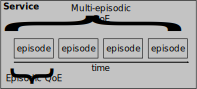
\includegraphics[width=1\columnwidth]{fig/multi-episodic}
	\caption{Repeated usage episodes with one service and their episodic QoE form a multi-episodic QoE in the user.}
	\label{img:chap01:multi-episodic}
\end{figure}

This thesis has two goals:
\paragraph*{Goal 1}
First, I will investigate what affects a retrospective multi-episodic quality judgment.
The major focus here is to understand which usage episode are of special importance for a multi-episodic quality judgment and what temporal effects occur.

\paragraph*{Goal 2}
Second, I will investigate how multi-episodic quality can be predicted based upon episodic quality judgments and investigate components for model.

\section{Structure}
This thesis is divided into two parts.
In \emph{Part I} I will introduce concepts and fundamentals that form the basis for my approach towards multi-episodic quality.
In Chapter~\ref{chap:02} an introduction on \ac{QoE} is given.
This includes prior work on psychophysics, perception and the quality formation process.
At the end of this chapter the relationship to higher level concepts like satisfaction and service quality is discussed.
In Chapter~\ref{chap:03} I present relevant concepts that affect recall and thus retrospective judgments of an \emph{general experience}.
Here, I will discuss how memory affects those retrospective judgments and those (temporal) effects are presented.
Based upon Chapter~\ref{chap:02} and Chapter~\ref{chap:03} I will present the state-of-the-art on performance fluctuations on QoE in one usage episode in Chapter~\ref{chap:04}.
This chapter closes with a review on found temporal effects in this domain and what how those effects are modeled.

In \emph{Part II} multi-episodic QoE is presented.
First an overview on prior work on multi-episodic QoE is given in Chapter~\ref{chap:05}.
Here the assessment methodology developed for multi-episodic QoE presented in \cite{moller_single-call_2011} is presented in detail.
This task-driven assessment methodology is 																													